%\noindent
\justifying
\setlength{\parskip}{1em}

To evaluate the quality of images generated by the \ac{CycleGAN}, a classifier is trained on the \ac{CycleGAN} generated data and its accuracy on a real dtest dataset is used as a metric to measure how well the \ac{CycleGAN} model distribution matches the real data distribution. Basically, The classification capability of the trained classifier is used as an objective measure to assess the quality of images generated by \ac{CycleGAN}.
Also, the classifier is trained on the synthetic document images and it's accuracy evaluated in 



Classification report and metrics



Three separate classifiers are trained upon synthetic data distribution, faxified data distribution, and \ac{CycleGAN} generated data distribution respectively. After training the classifiers they have evaluated annotated real document images. Using this performance evaluation using metrics like weighted f1 score and accuracy 	


\section{Evaluation Metrics}



\subsection{Accuracy}


\subsection{f1-score}


\section{Experiments}\label{experiments}


In this thesis, many experiments were performed to understand the domain gap between data distributions. Three data distributions are considered for the experiments. Each data distribution represents a different domain. The synthetic document images represent the synthetic data distribution. The faxified document images represent faxified data distribution. The \ac{CycleGAN} generated images represent \ac{CycleGAN} generated data distribution. The goal of the experiments is to illustrate and analyse the domain gap between the real data distribution and above mentioned three data distributions. Now let us explain steps involved while performing experiments. First, the classifier(figure \ref{fig:ClassifierArchitectureBlocks}) is trained on synthetic document images and its performance is evaluated on annotated real document images. Second, the new classifier with the same architecture is trained on faxified document images and its performance is evaluated on annotated real document images. Third, the \ac{CycleGAN} is trained using synthetic document images and real document images and at the end of every epoch, the checkpoint is saved. Once training is finished all saved checkpoints are loaded. The forward Generator $G$ is loaded and 100,000 synthetic document images are transformed into 100,000 realistic document images. The realistic document images are also referenced interchangeably as \ac{CycleGAN} generated images. Forward Generator $G$  transforms images from the source domain to the target domain where synthetic document images represent the source domain and real document images represent the target domain. Next, 100,000 \ac{CycleGAN} generated document images are used to train another new classifier with the same architecture as the previous, and its performance is evaluated on annotated real document images. The experiment aims to understand the quality of the images generated by \ac{CycleGAN}. Especially, how efficiently \ac{CycleGAN} was able to close the domain gap between synthetic data distribution and real data distribution. The evaluation metrics like accuracy, weighted average F1 score, and macro average F1 score \cite{lipton2014thresholding} are used to understand the contrast between the performance of the classifiers on annotated real document images.

\subsection{Experiment Steps}


\begin{enumerate}

    \itemsep0em 
    \item Train a classifier on synthetic document images and evaluate its classification performance on the annotated real document images.
    \item Train a classifier on faxified document images and evaluate its classification performance on the annotated real document images.
    \item Train a \ac{CycleGAN}.
    \item Generate document images using trained \ac{CycleGAN}. 
    \item Train a classifier on \ac{CycleGAN} generated document images and  evaluate its classification performance on the annotated real document images.
    \item Compare the classification performance of the above three classifiers on the annotated real document images to illustrate the domain gap between real data distribution and three distributions synthetic data, faxified data, and \ac{CycleGAN} generated data.

\end{enumerate}




\subsection{\ac{CycleGAN} Training}

The \ac{CycleGAN} consists of two generators $G$ and $F$ and two discriminators $D_X$ and $D_Y$. Domain $X$ represents Source Domain and Domain $Y$ represents Target Domain. The aim is to transform Synthetic Document Images into Realistic Document Images. Hence, The Synthetic Document Images represent the Source Domain and Real Document Images represent the Target Domain.




\begin{comment}

\begin{figure}[H]
  \centering
  \begin{minipage}[b]{0.49\textwidth}
    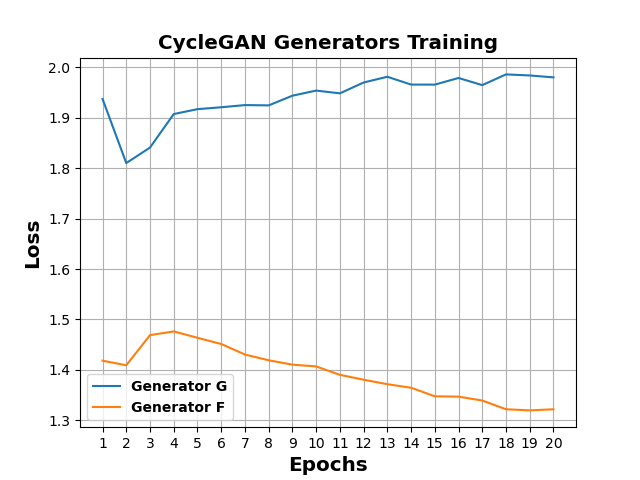
\includegraphics[width=\textwidth]{images/CycleGAN_Generators_Training.png}
    \caption[Epoch vs Loss Plot. \ac{CycleGAN} Generators $G$ and $F$ Training.]{Epoch vs Loss Plot. \ac{CycleGAN} Generators $G$ and $F$ Training.}
    \label{fig:CycleGANGeneratorsTraining}
  \end{minipage}
  \hfill
  \begin{minipage}[b]{0.49\textwidth}
    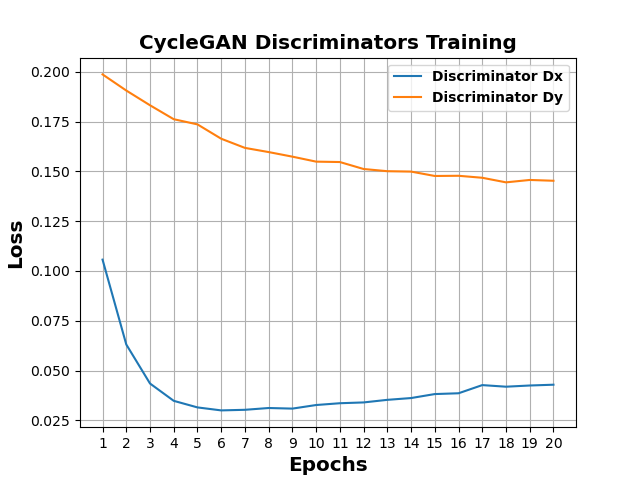
\includegraphics[width=\textwidth]{images/CycleGAN_Discriminators_Training.png}
    \caption[Epoch vs Loss Plot. \ac{CycleGAN} Discriminators Training.]{Epoch vs Loss Plot. \ac{CycleGAN} Discriminators $D_X$ and $D_Y$ Training.}
    \label{fig:CycleGANDiscriminatorsTraining}
  \end{minipage}
\end{figure}



\begin{figure}[H]
  \centering
  \begin{minipage}[b]{0.49\textwidth}
    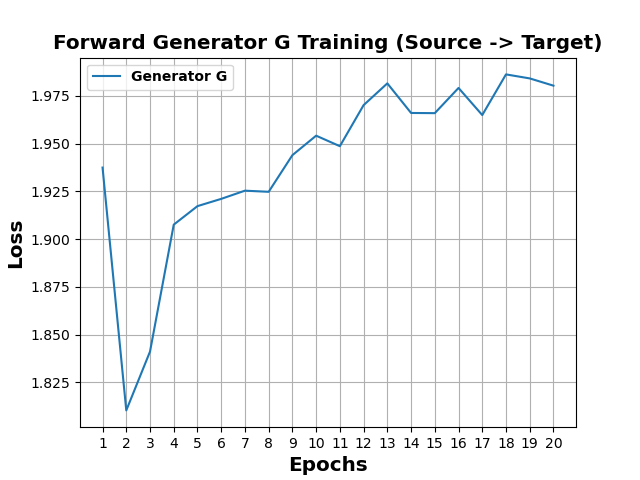
\includegraphics[width=\textwidth]{images/Generator_G_Training.png}
    \caption[Epoch vs Loss Plot. \ac{CycleGAN} Forward Generator $G$ Training.]{Epoch vs Loss Plot. \ac{CycleGAN} Forward Generator $G$ Training. }
    \label{fig:generatorG}
  \end{minipage}
  \hfill
  \begin{minipage}[b]{0.49\textwidth}
    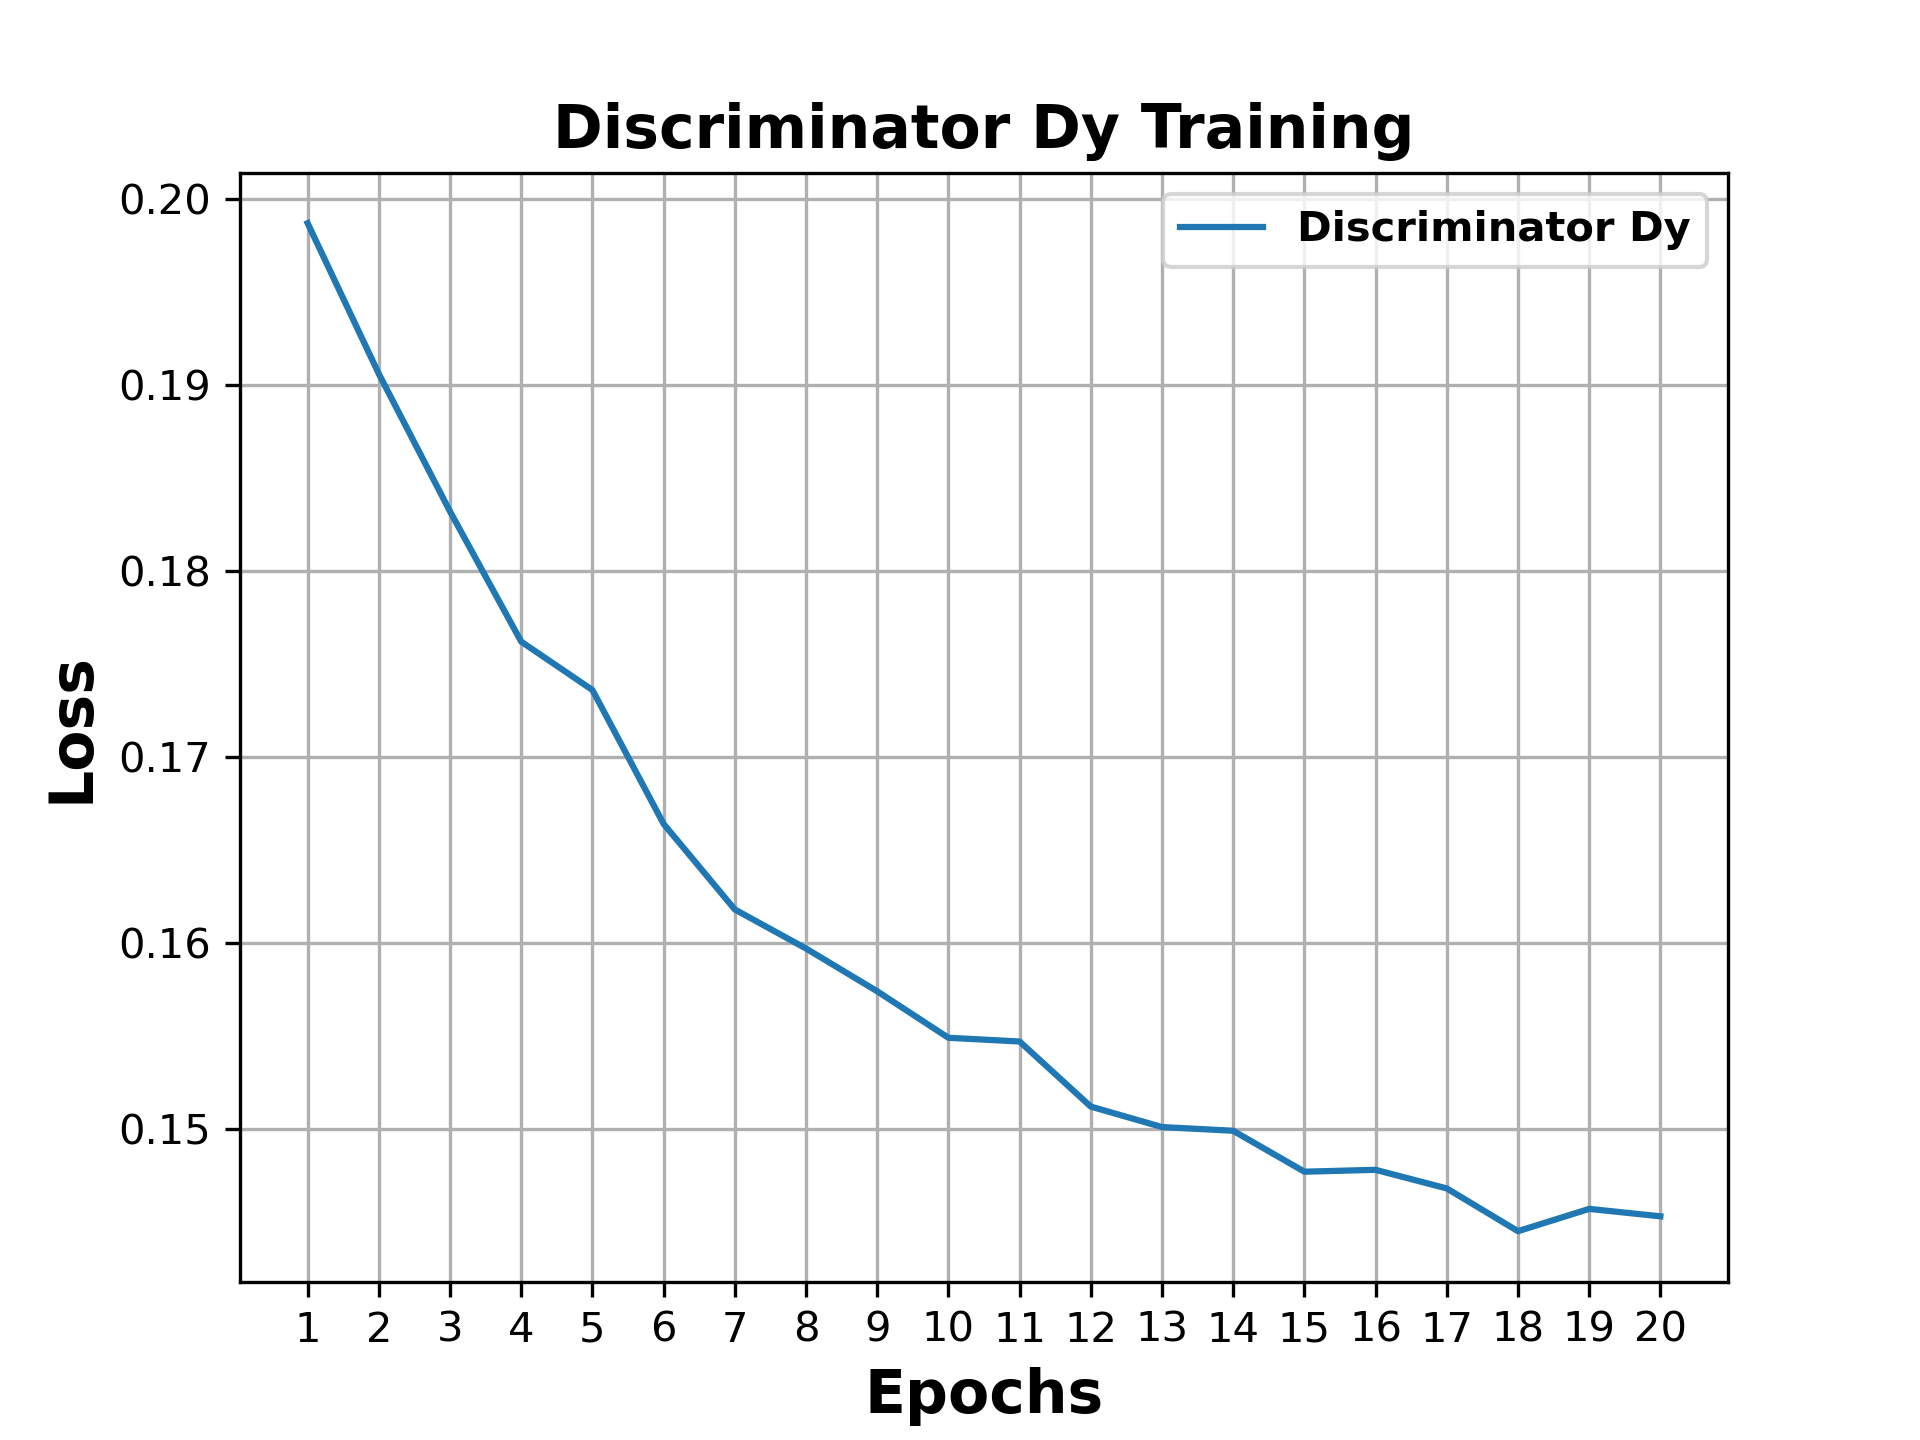
\includegraphics[width=\textwidth]{images/Discriminator_Dy_Training.png}
    \caption[Epoch vs Loss Plot. \ac{CycleGAN} Discriminator $D_Y$ Training.]{Epoch vs Loss Plot. \ac{CycleGAN} Discriminator $D_Y$ Training. }
    \label{fig:discriminatorDy}
  \end{minipage}
\end{figure}






\begin{figure}[H]
  \centering
  \begin{minipage}[b]{0.49\textwidth}
    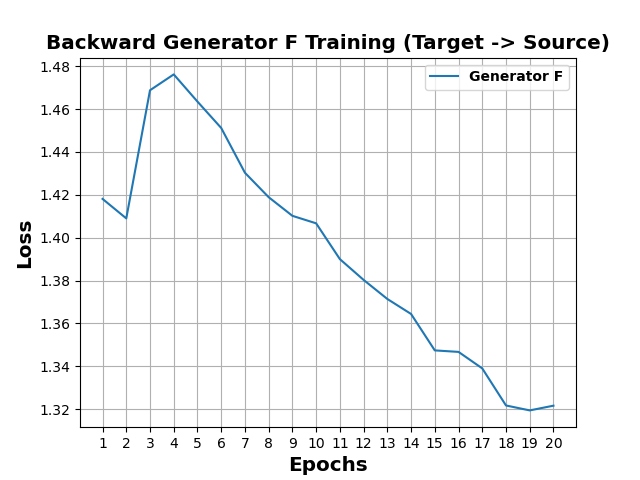
\includegraphics[width=\textwidth]{images/Generator_F_Training.png}
    \caption[Epoch vs Loss Plot. \ac{CycleGAN} Backward Generator $F$ Training.]{Epoch vs Loss Plot. \ac{CycleGAN} Backward Generator $F$ Training.}
    \label{fig:generatorF}
  \end{minipage}
  \hfill
  \begin{minipage}[b]{0.49\textwidth}
    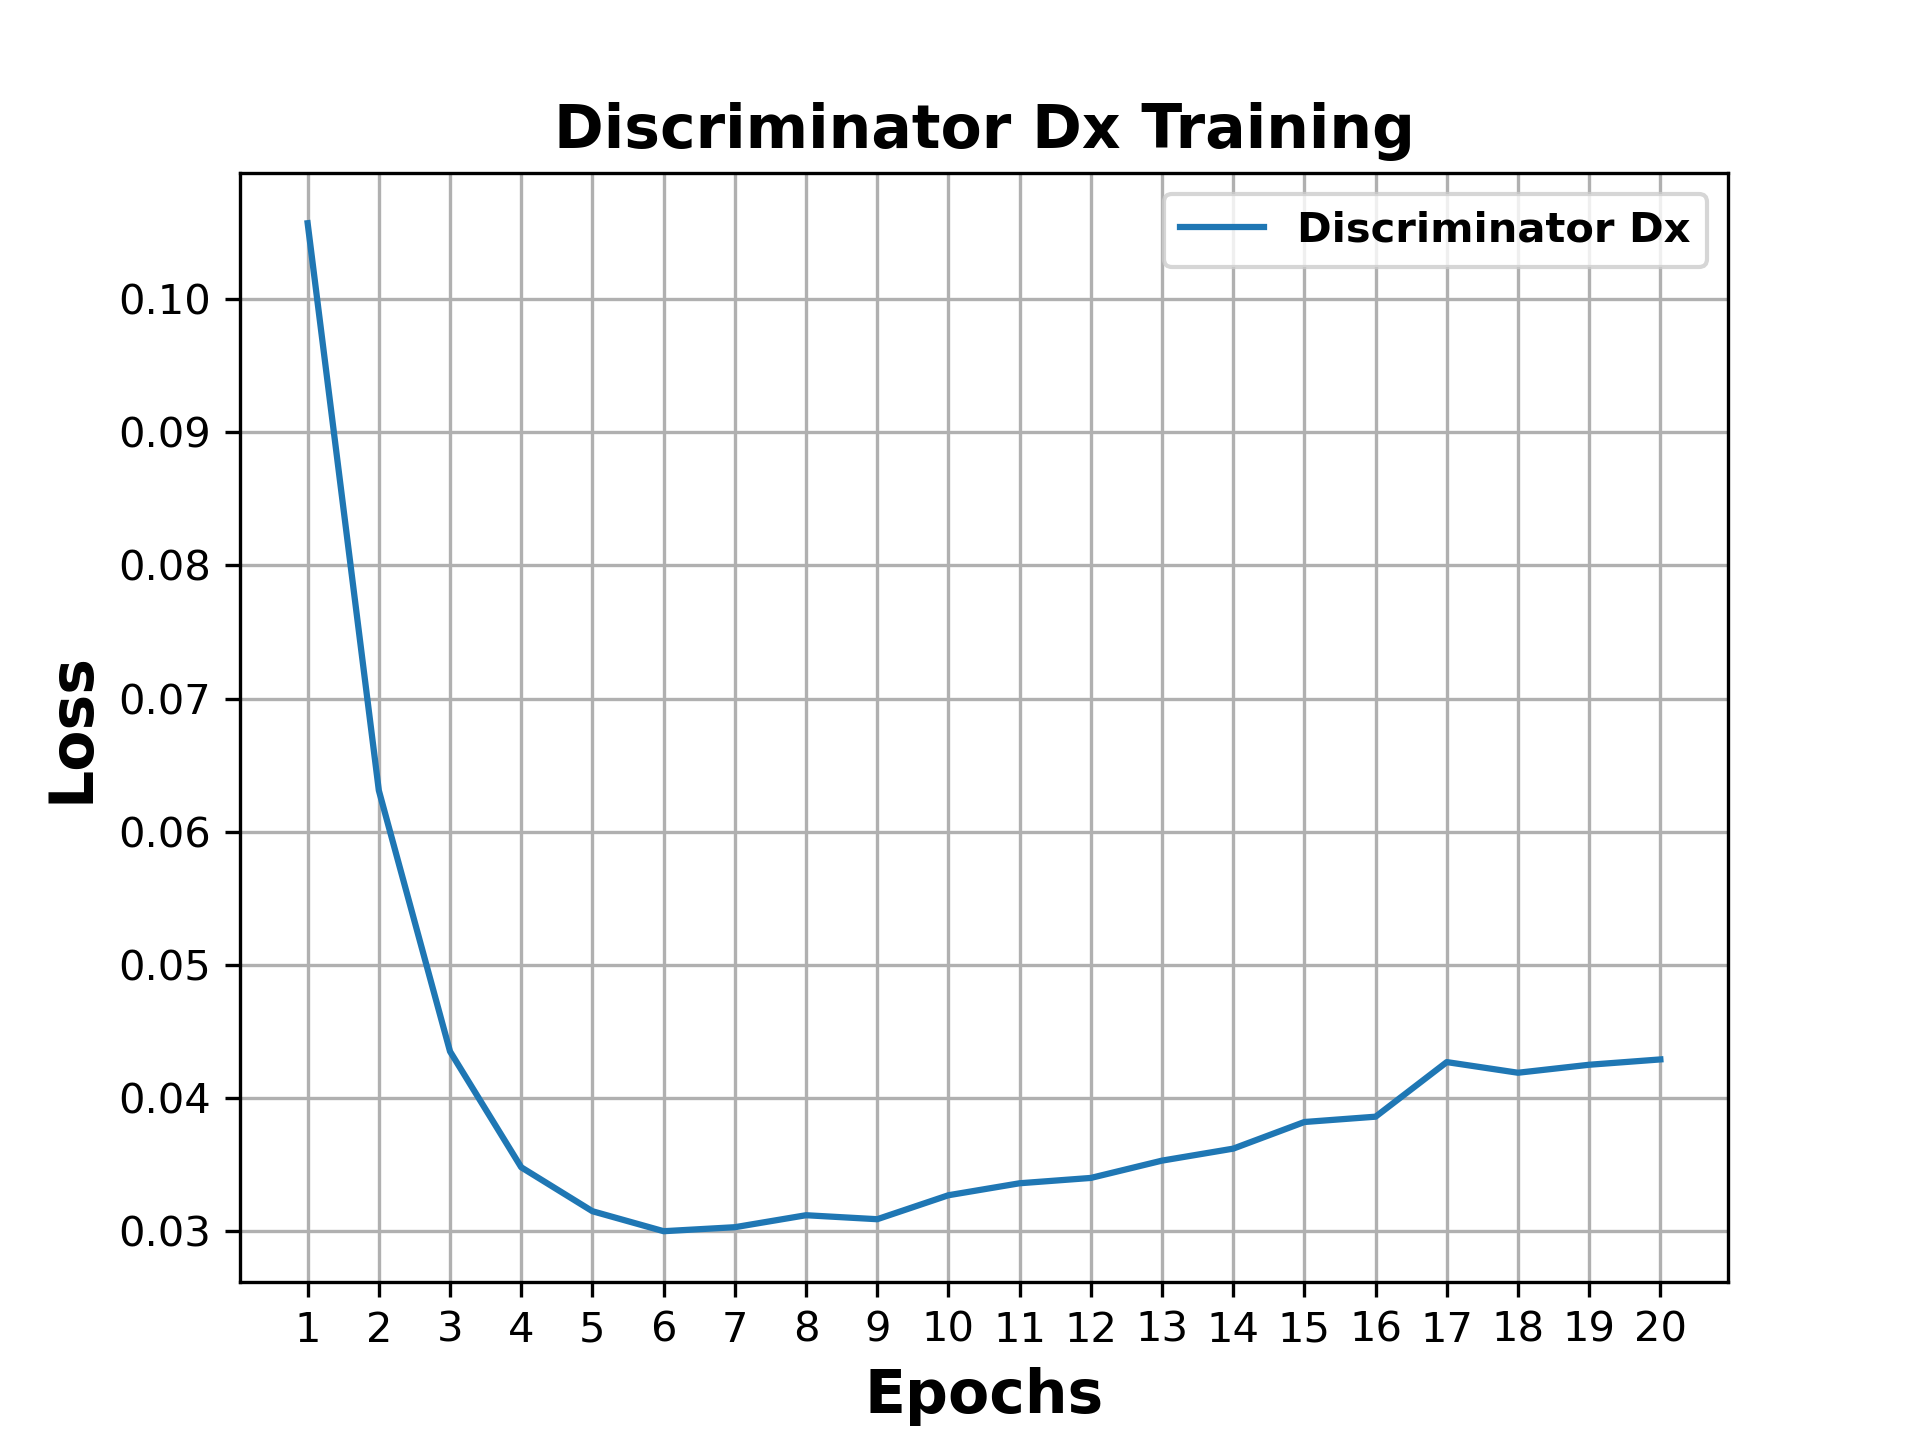
\includegraphics[width=\textwidth]{images/Discriminator_Dx_Training.png}
    \caption[Epoch vs Loss Plot. \ac{CycleGAN} Discriminator $D_X$ Training.]{Epoch vs Loss Plot. \ac{CycleGAN} Discriminator $D_X$ Training.}
    \label{fig:discriminatorDx}
  \end{minipage}
\end{figure}

\end{comment}





\subsection{Training a Classifier on Synthetic Document Images}\label{trainingsyntheticclassifier}



\begin{figure}[H]
  \centering
  \begin{minipage}[b]{0.49\textwidth}
    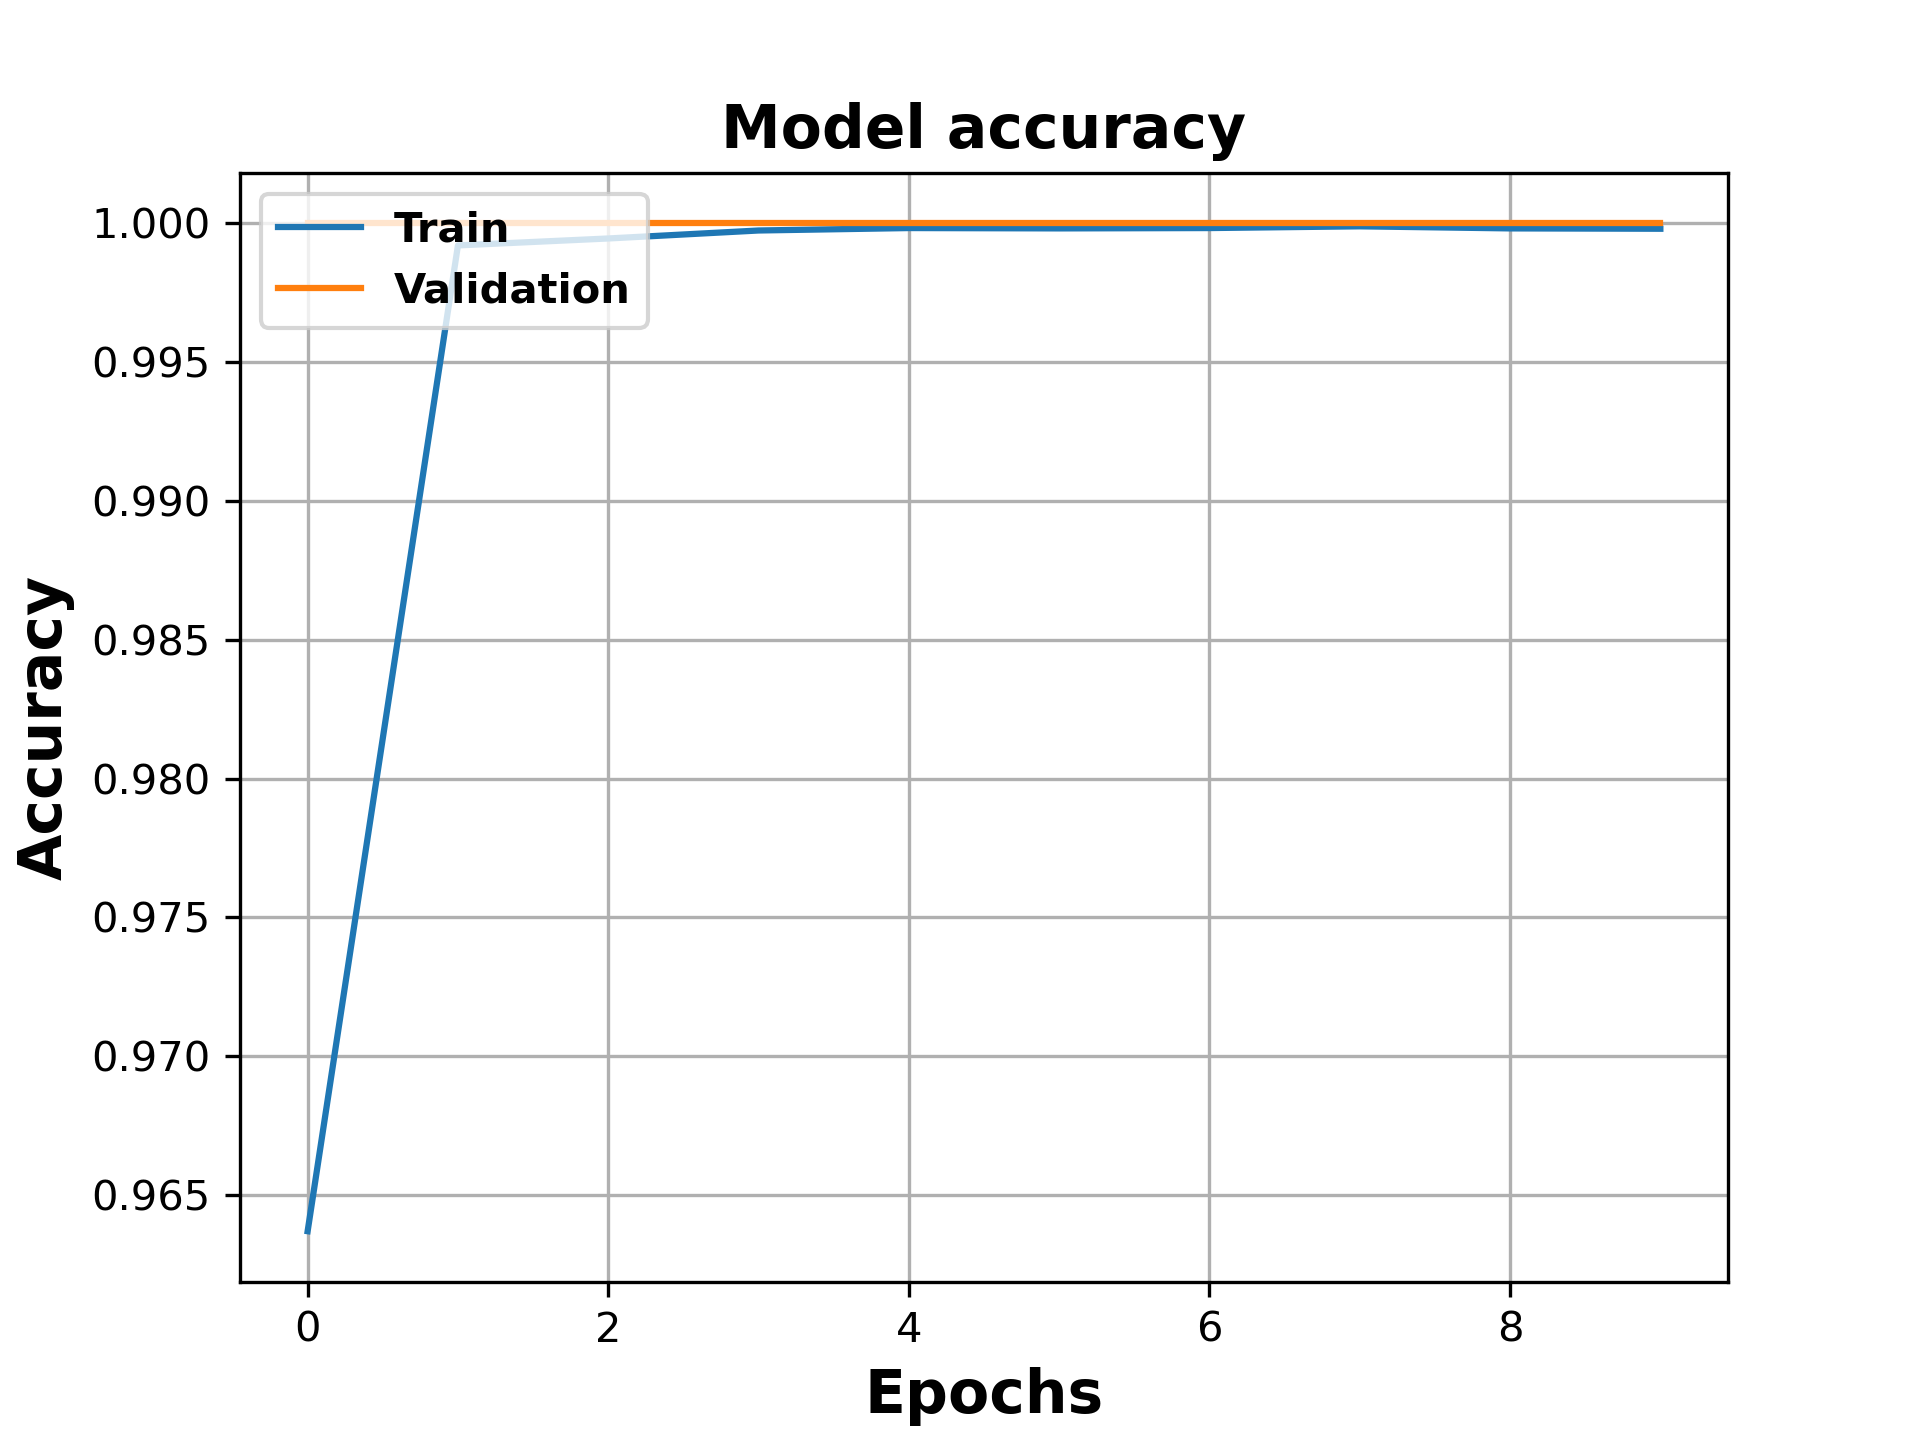
\includegraphics[width=\textwidth]{images/Synthetic_Data_Classifier_2021-05-21_13-52-04_Accuracy.png}
    \caption[Epoch vs Accuracy Plot. Training the Classifier on Synthetic Document Images.]{Epoch vs Accuracy. Training the Classifier on Synthetic Document Images.}
    \label{fig:SyntheticClassifierAcc}
  \end{minipage}
  \hfill
  \begin{minipage}[b]{0.49\textwidth}
    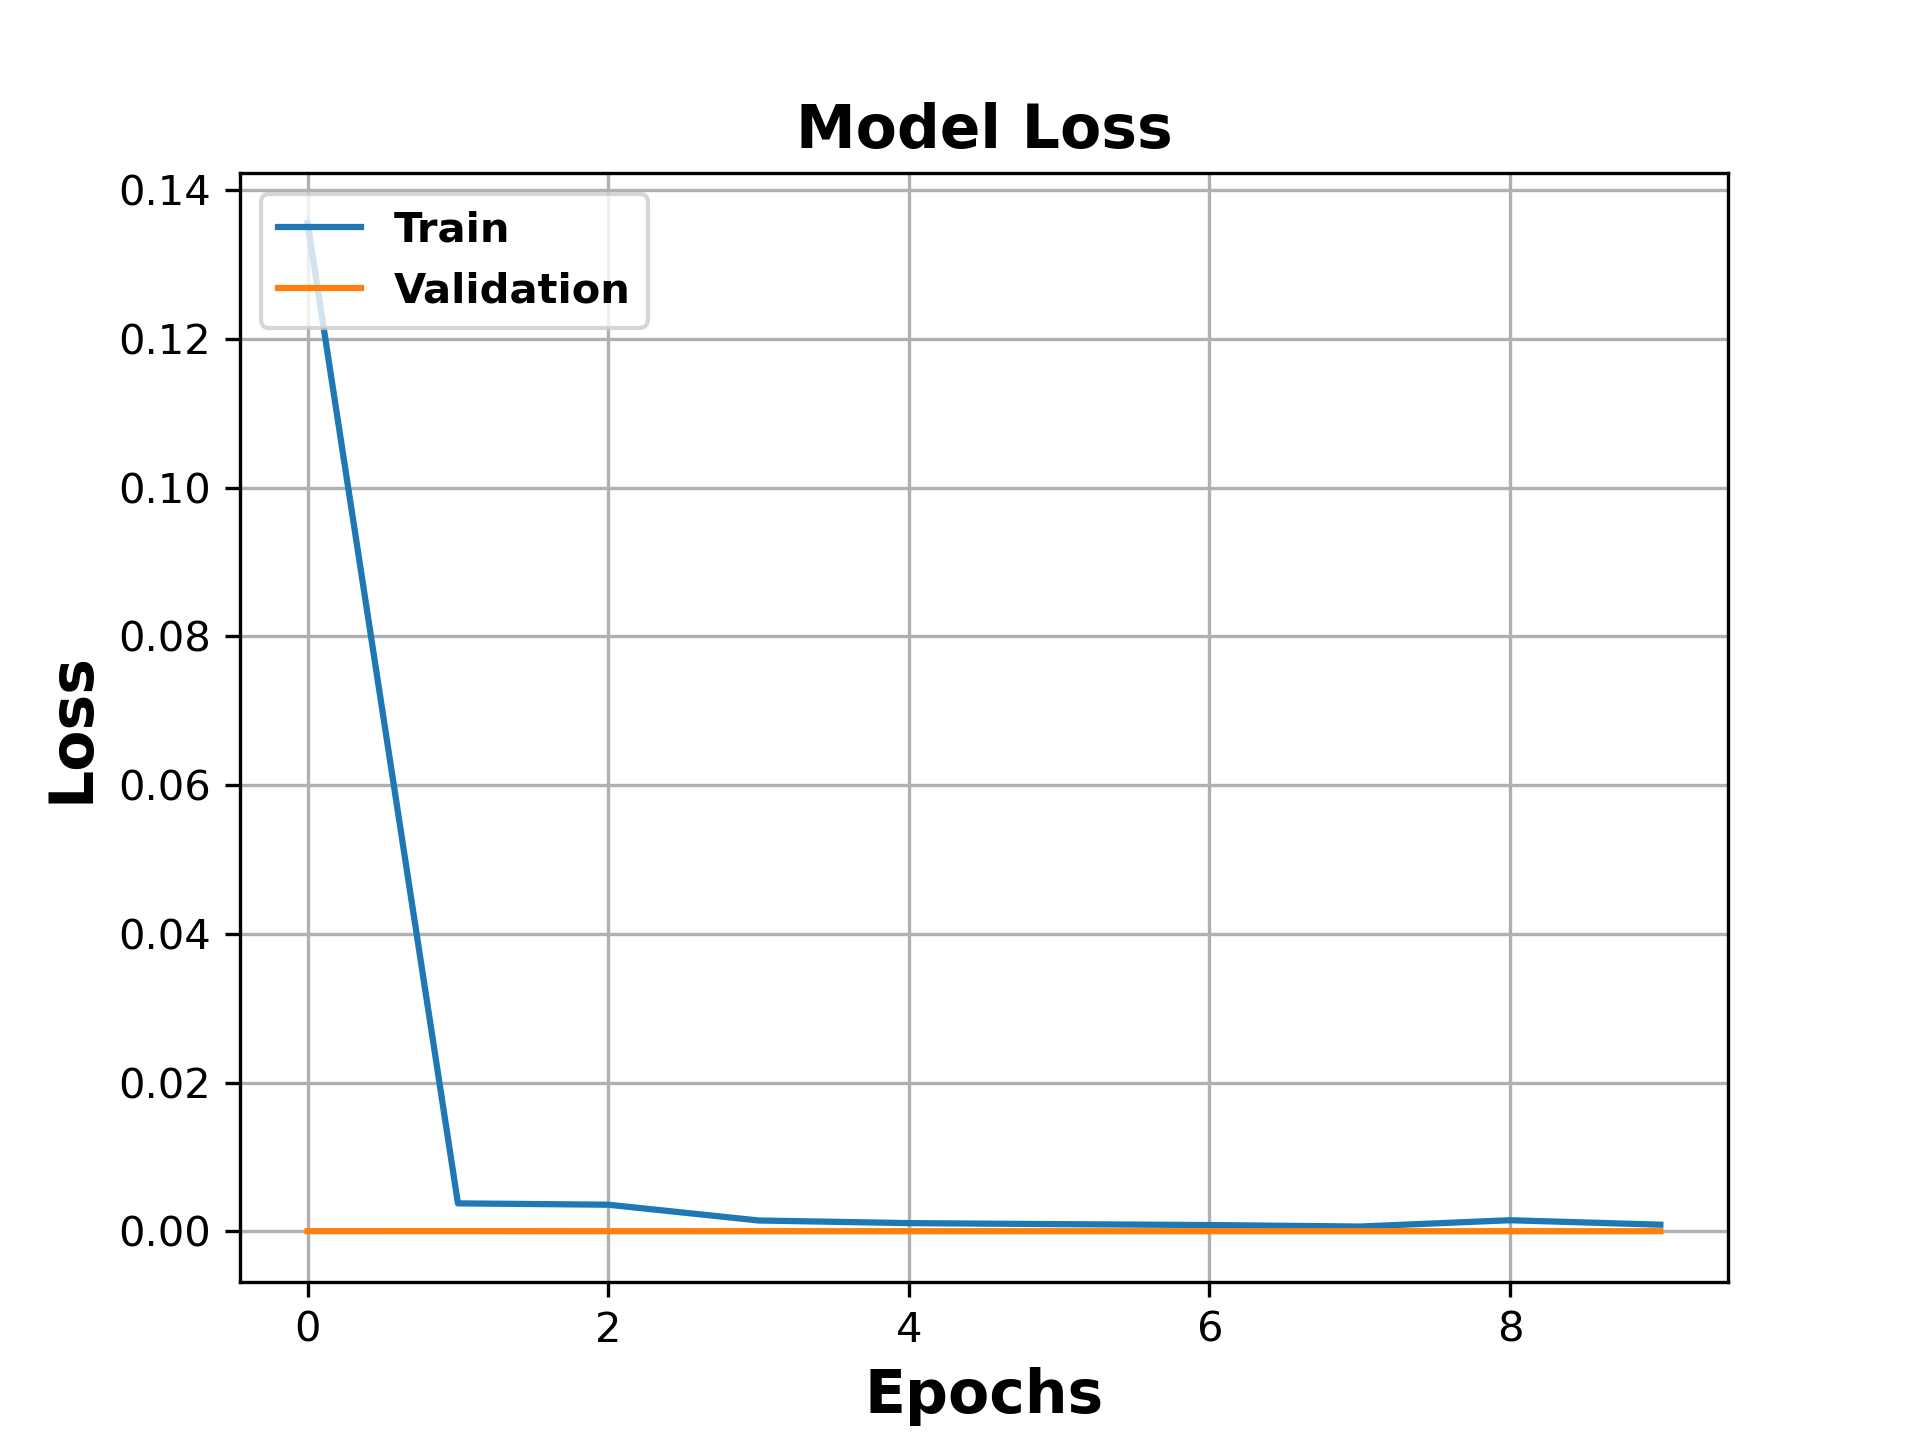
\includegraphics[width=\textwidth]{images/Synthetic_Data_Classifier_2021-05-21_13-52-04_Loss.png}
    \caption[Epoch vs Loss Plot. Training the Classifier on Synthetic Document Images.]{Epoch vs Loss Plot. Training the Classifier on Synthetic Document Images.}
    \label{fig:SyntheticClassifierLoss}
  \end{minipage}
\end{figure}


\begin{center}
\begin{table}[H]
    \begin{center}
    \begin{tabular}{p{0.22\linewidth} p{0.10\linewidth} p{0.10\linewidth} p{0.10\linewidth} p{0.10\linewidth}} 
        \toprule
            & Precision & Recall & F1-score & Support\\[0.0ex] 
        \midrule
        DE\_LY\_Arm\_2020-01 & 0.84 & 0.48 & 0.61 & 44\\[0.0ex]
        \midrule
        DE\_LY\_Bein\_2018-08 & 0.07 & 0.49 & 0.12 & 47\\[0.0ex]
        \midrule
        DE\_LY\_Bein\_2019-01 & 0.23 & 0.22 & 0.23 & 50\\[0.0ex]
        \midrule
        DE\_LY\_Bein\_2019-07 & 0.22 & 0.43 & 0.29 & 60\\[0.0ex]
        \midrule
        DE\_LY\_Bein\_2020-01 & 0.86 & 0.23 & 0.36 & 624\\[0.0ex]
        \midrule
        DE\_LY\_Bein\_2020-03 & 0.23 & 0.19 & 0.21 & 128\\[0.0ex]
        \midrule
        DE\_LY\_Hand\_2020-01 & 0.92 & 0.69 & 0.79 & 16\\[0.0ex]
        \midrule
        DE\_PH\_Bein\_2018-09 & 0.16 & 0.23 & 0.19 & 22\\[0.0ex]
        \midrule
        DE\_PH\_Bein\_2019-02 & 0.10 & 0.21 & 0.14 & 28\\[0.0ex]
        \midrule
        DE\_PH\_Bein\_2020-01 & 0.28 & 0.51 & 0.36 & 143\\[0.0ex]
        \midrule
        \midrule
        Accuracy              &      &      & \bf{0.30} & 1162\\[0.0ex]
        Macro Average             & 0.39 & 0.37 & 0.33 & 1162\\[0.0ex]
        Weighted Average          & 0.59 & 0.30 & 0.33 & 1162\\[0.0ex]
        \bottomrule
    \end{tabular}
    \caption{Classification Report. The Classifier is trained On Synthetic Document Images, its Classification Performance Evaluated on the Annotated Real Document Images.}
    \label{table:SyntheticClassificationReport}
    \end{center}
\end{table}
\end{center}



\subsection{Training a Classifier on \ac{CycleGAN} Generated Document Images}














\subsection{Training a Classifier on Faxified Document Images}\label{trainingfaxifiedclassifier}

The faxification process mimics the way the fax machine works. It transforms the images in such a way like it was sent via fax. Whi


Usually, fax machines use a horizontal resolution of 1728 pixels and transmit only black-and-white images, which might be dirty and are generally also not aligned perfectly. The faxification process is not deterministic, involves randomness during the process of faxification of the images.  It uses several image transformations like gamma, brightness, rotations, resizing, rescaling, binarization, adding noise, adding verticle lines, and conversion to a grayscale image. In figure \ref{fig:FaxificationProcessZoomed}, it is visible a snippet from the synthetic document image that has transformed randomly when it has been through the faxification process. 

\begin{figure}[H]
        \begin{center}
	    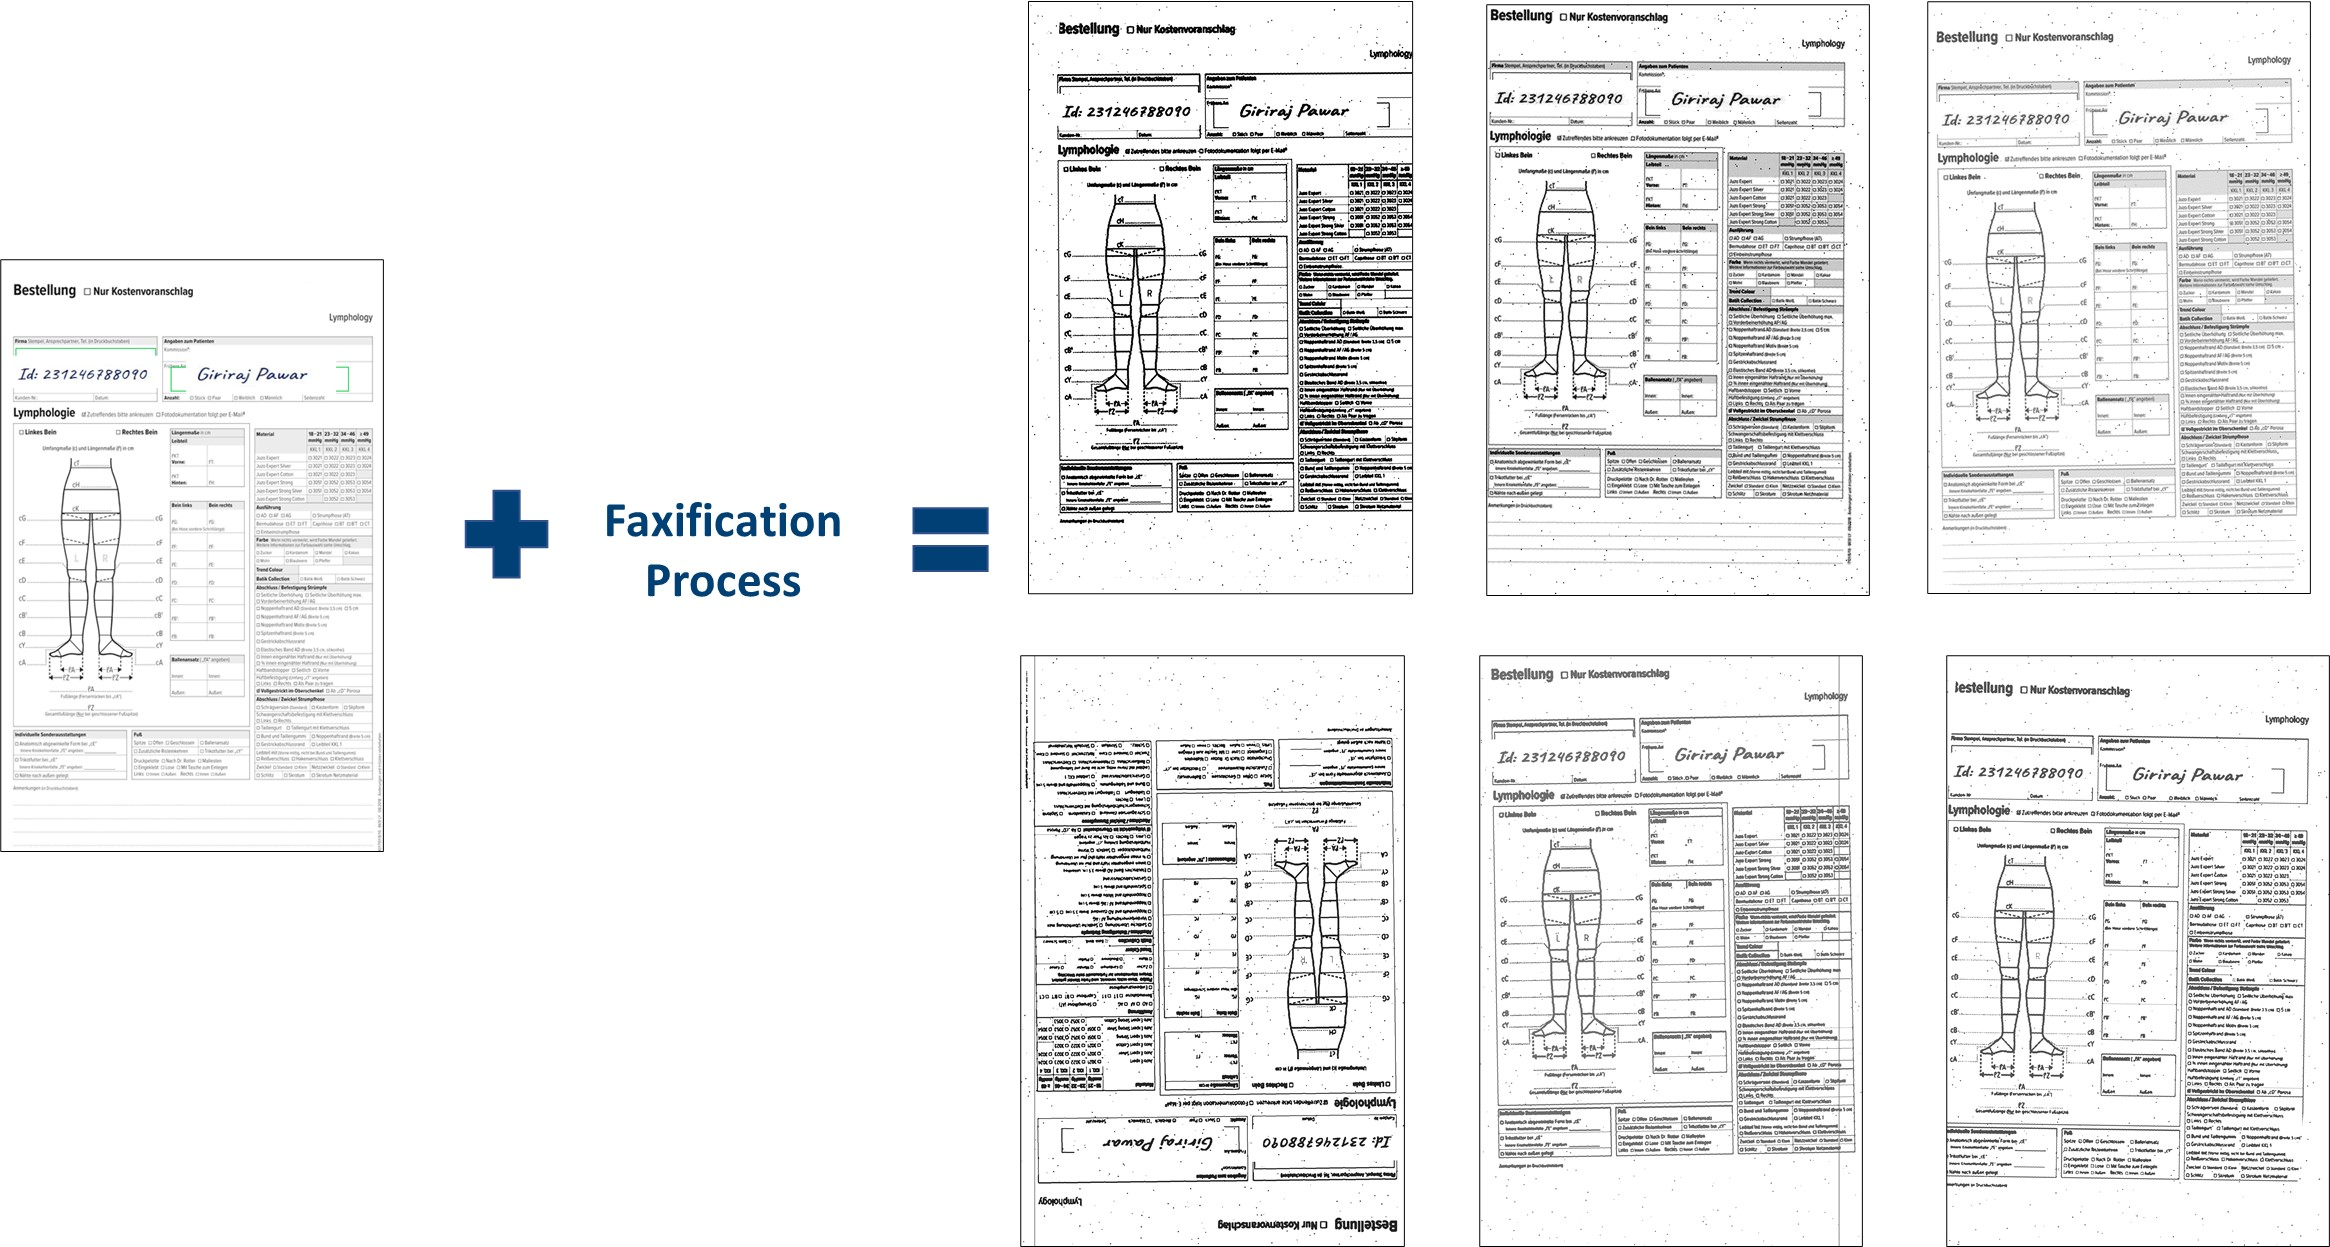
\includegraphics[scale=0.25]{images/FaxificationProcess.jpg}
	    \caption[Illustration of Faxification Process Applied on Synthetic Document Images.]{Illustration of Faxification Process Applied on Synthetic Document Images.}
	    \label{fig:FaxificationProcess}
	    \end{center}
\end{figure}



\begin{figure}[H]
        \begin{center}
	    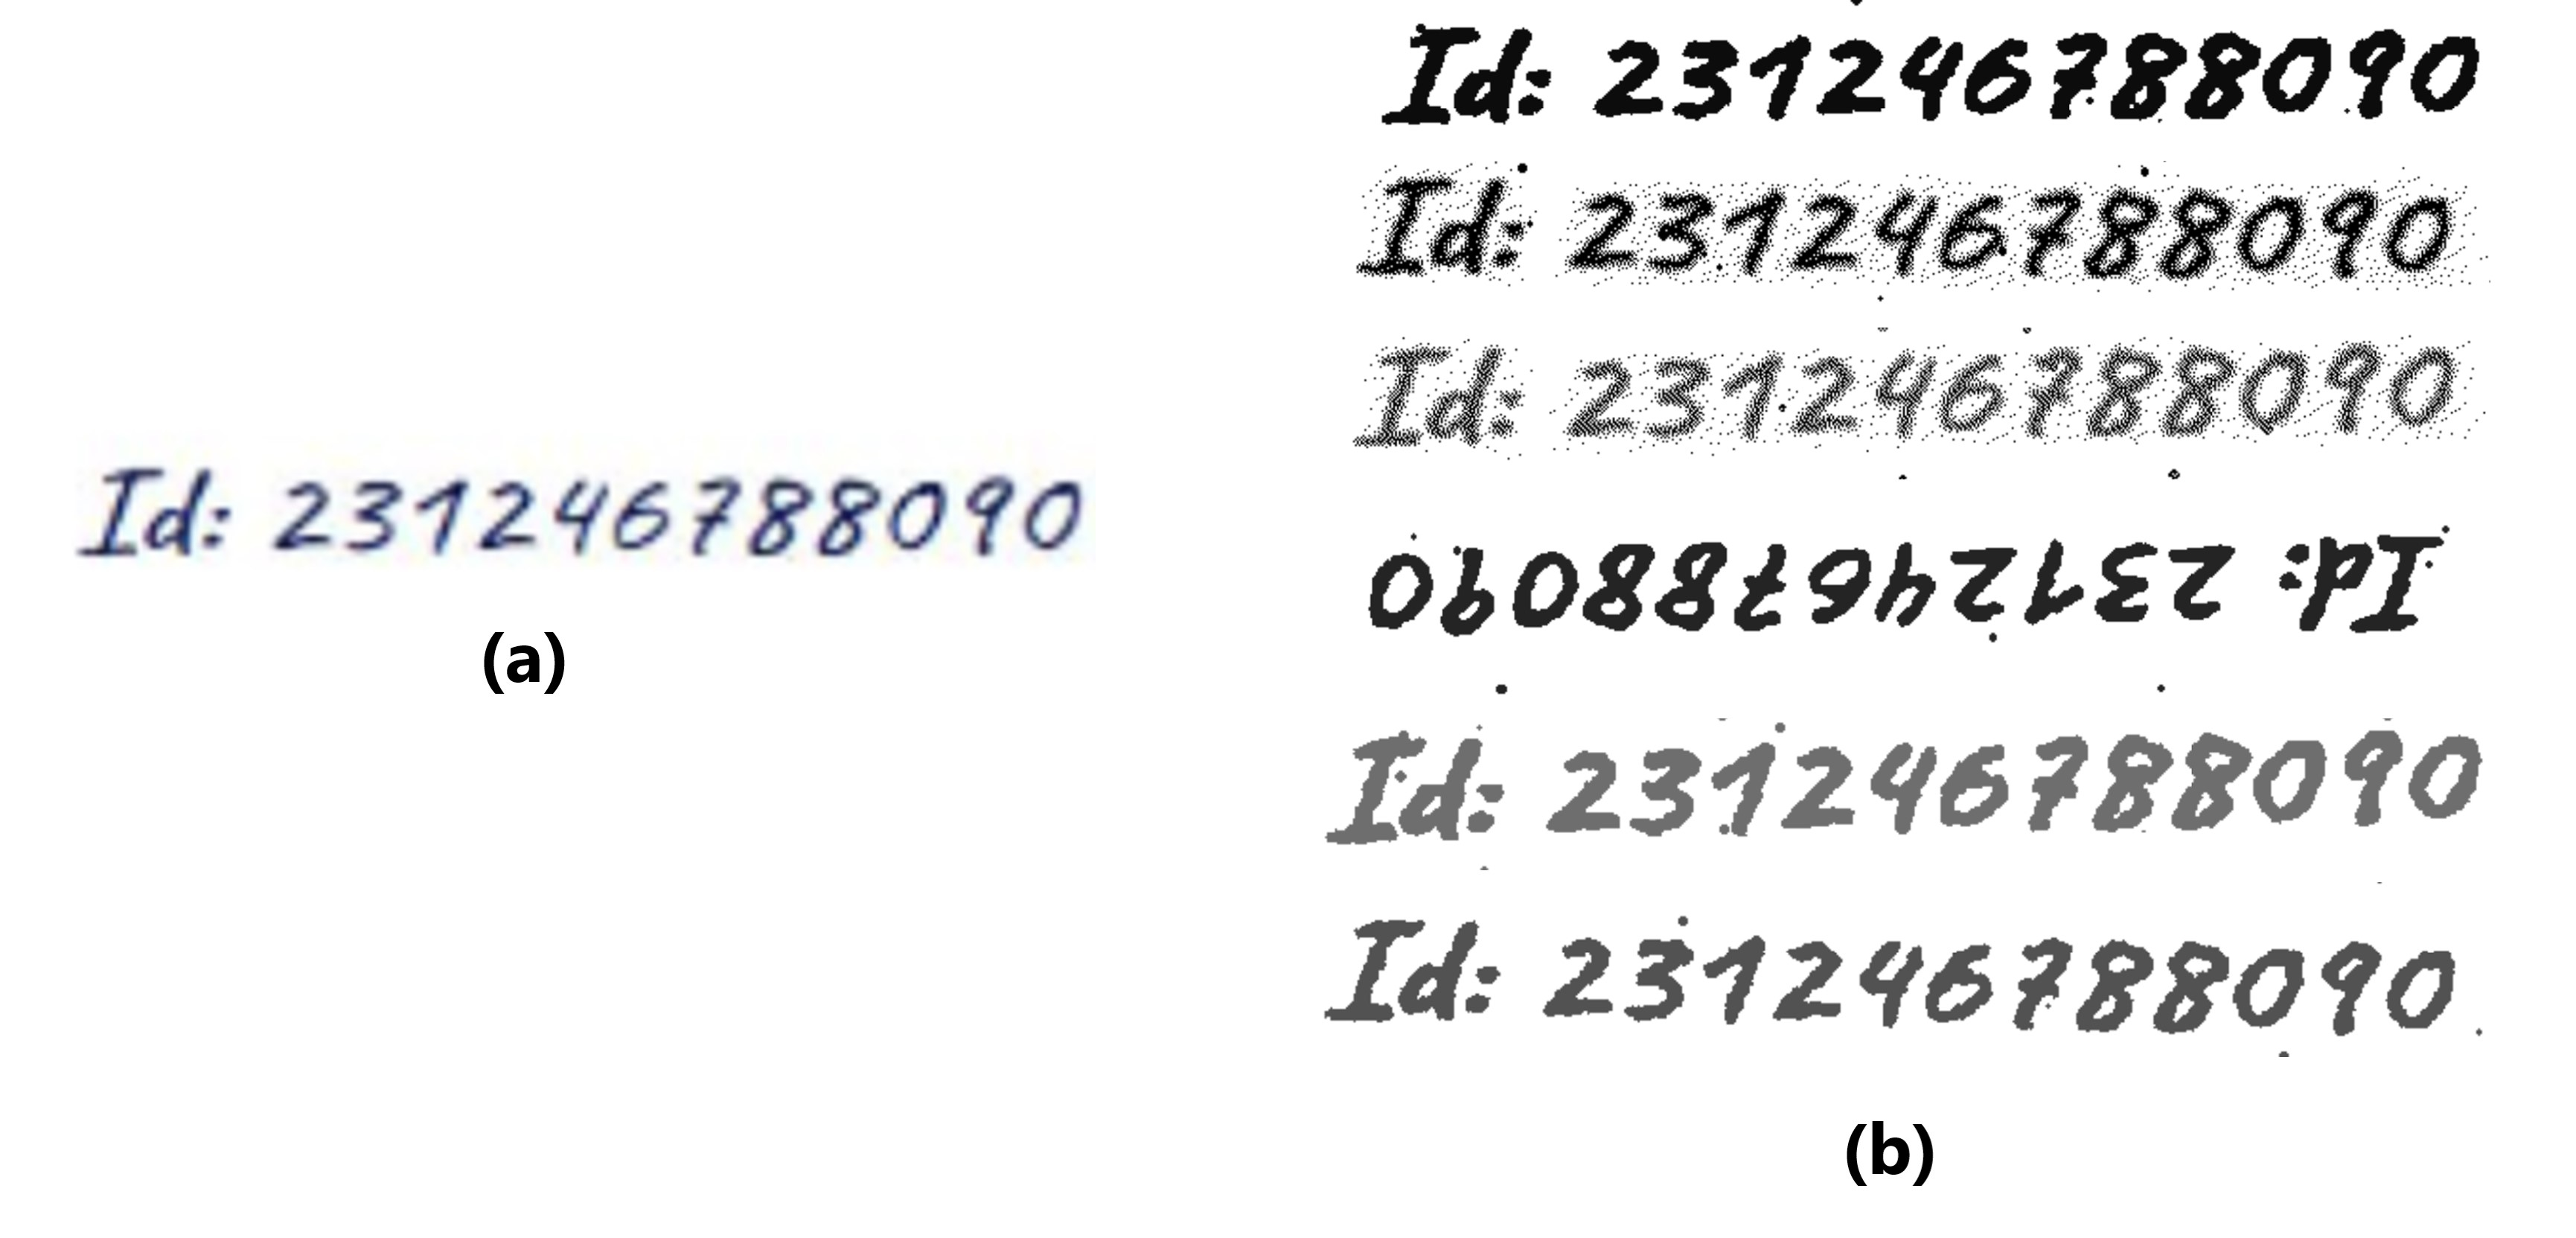
\includegraphics[scale=0.15]{images/FaxificationProcessZoomed.jpg}
	    \caption[Illustration of faxified images.]{Illustration of faxified images to conclude that faxification process is a random process, the input images are faxified randomaly to create distinct output. For example, snippets shown in (b) for a single type of image snippet in (a) are distinct and random. (a) Snippet from the synthetic document image. (b) Snippets from the faxified document images.}
	    \label{fig:FaxificationProcessZoomed}
	    \end{center}
\end{figure}




\begin{figure}[H]
  \centering
  \begin{minipage}[b]{0.49\textwidth}
    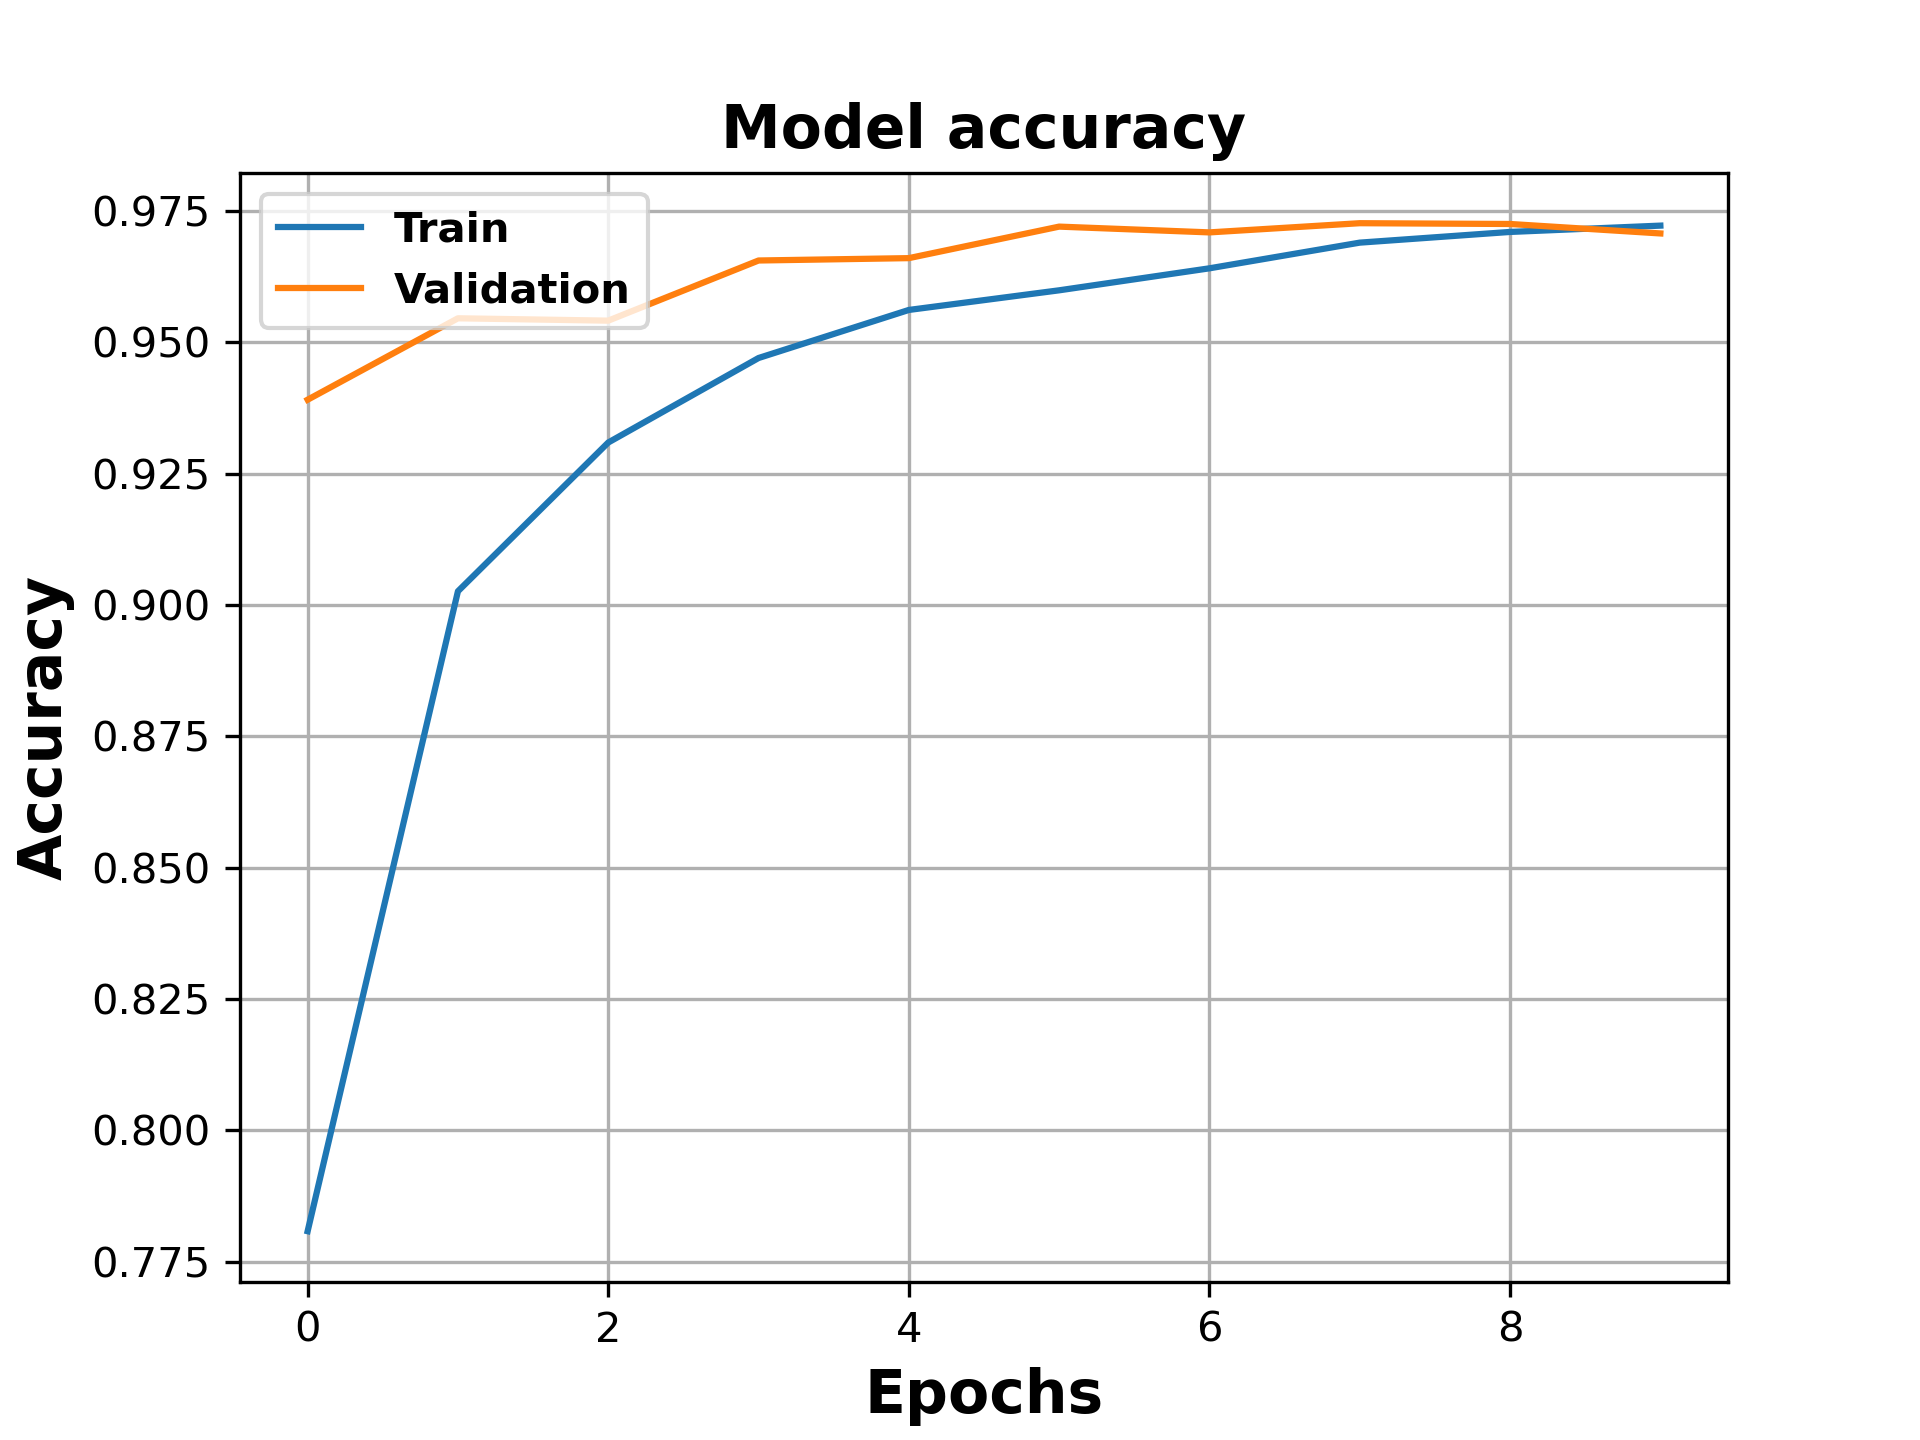
\includegraphics[width=\textwidth]{images/Faxifier_Data_Classifier_2021-05-21_13-50-07_Accuracy.png}
    \caption[Epoch vs Accuracy Plot. Training the Classifier on Faxified Document Images.]{Epoch vs Accuracy Plot. Training the Classifier on Faxified Document Images.}
    \label{fig:FaxifiedClassifierAcc}
  \end{minipage}
  \hfill
  \begin{minipage}[b]{0.49\textwidth}
    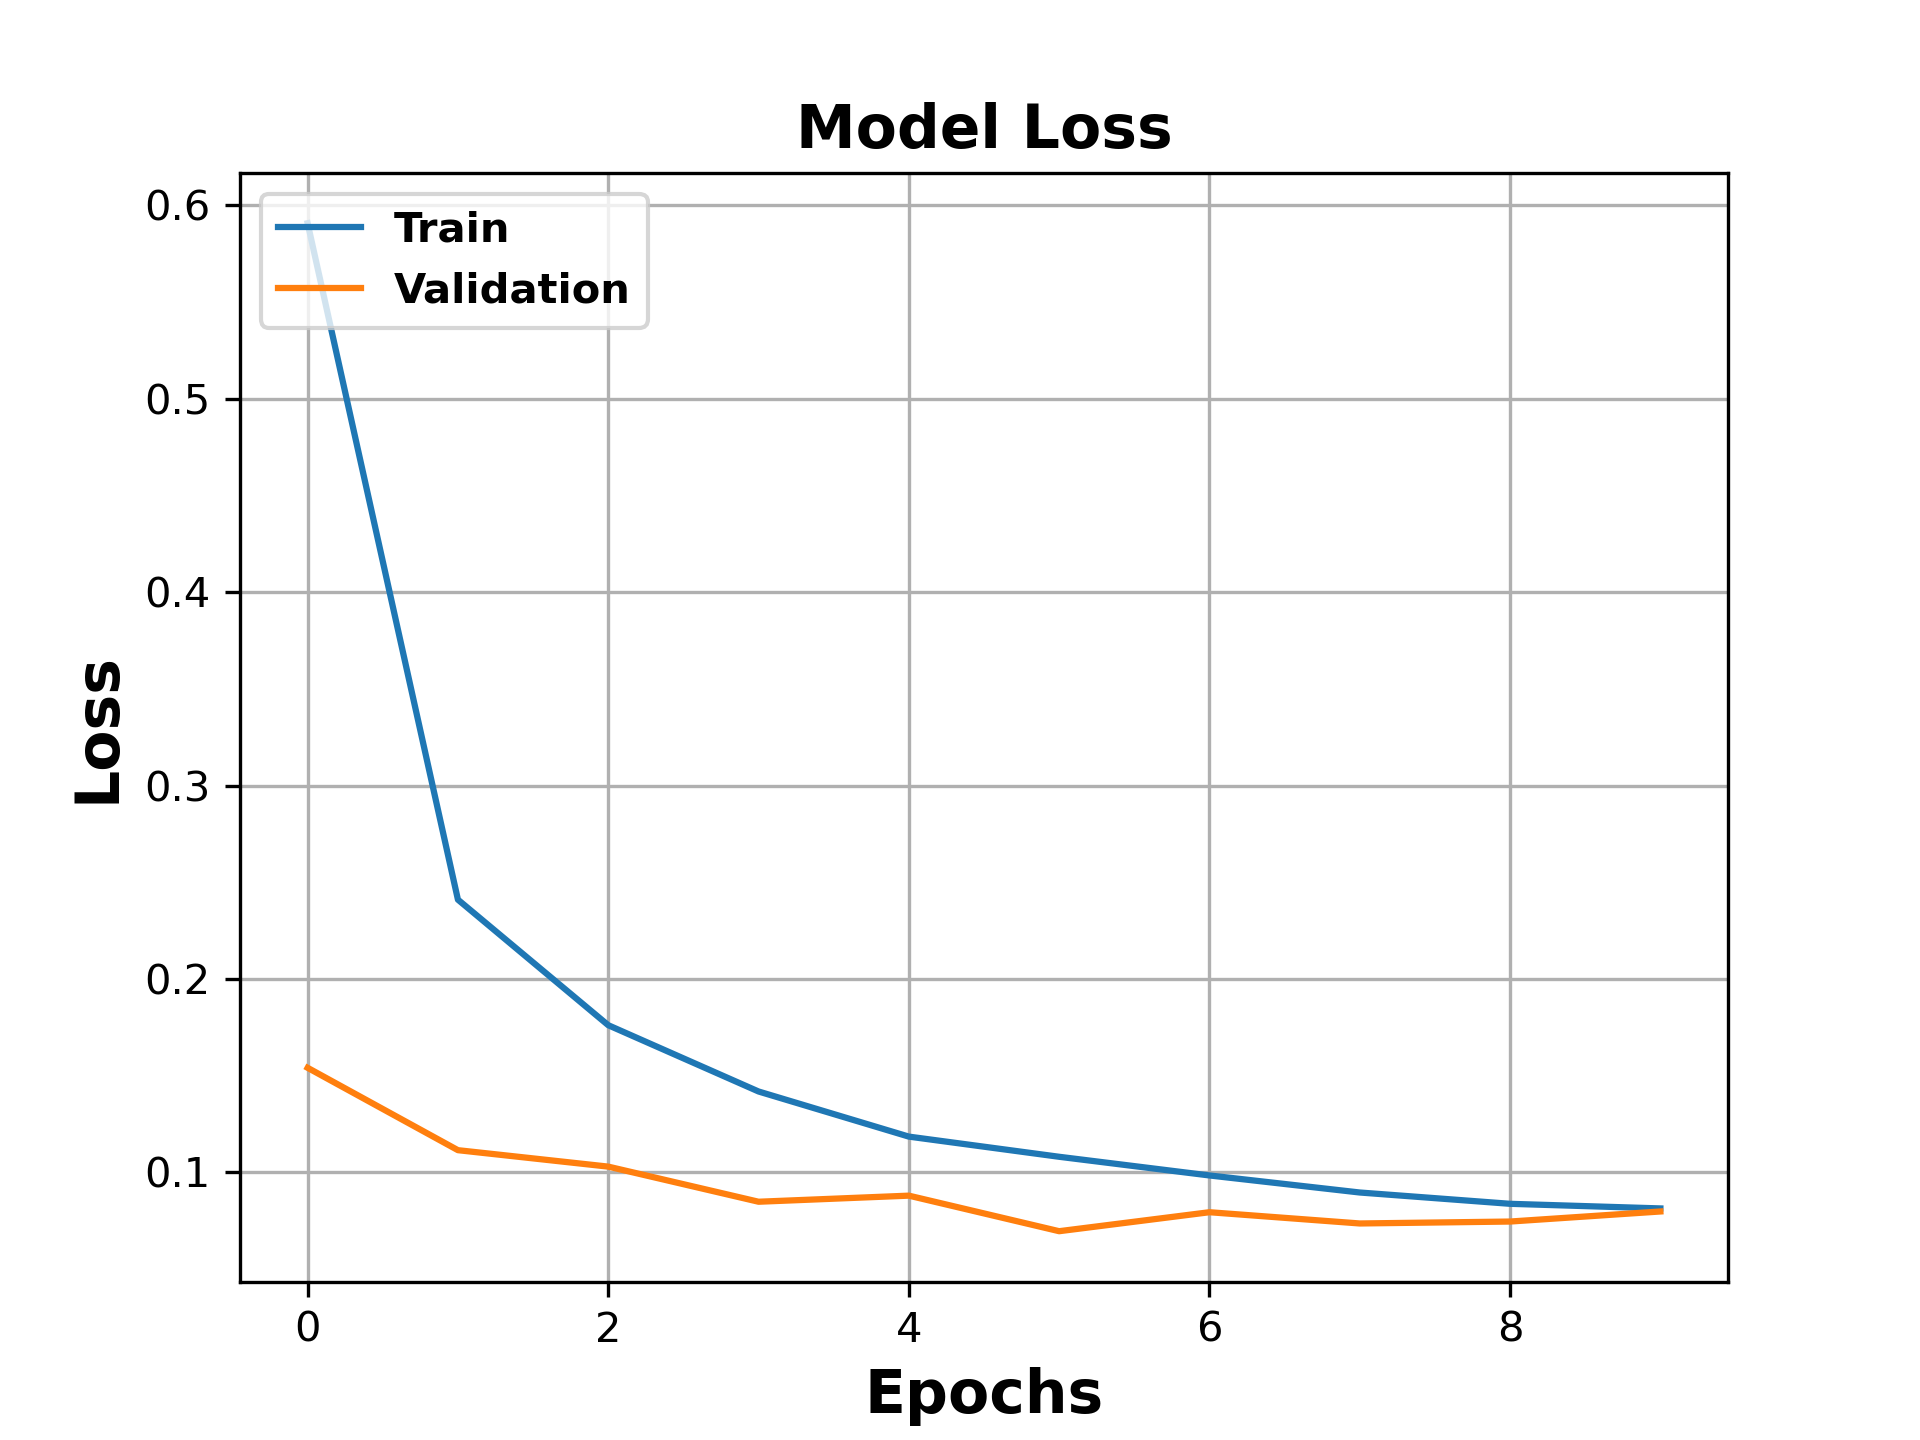
\includegraphics[width=\textwidth]{images/Faxifier_Data_Classifier_2021-05-21_13-50-07_Loss.png}
    \caption[Epoch vs Loss Plot. Training the Classifier on Faxified Document Images.]{Epoch vs Loss Plot. Training the Classifier on Faxified Document Images.}
    \label{fig:FaxifiedClassifierLoss}
  \end{minipage}
\end{figure}




\begin{center}
\begin{table}[H]
    \begin{center}
    \begin{tabular}{p{0.22\linewidth} p{0.10\linewidth} p{0.10\linewidth} p{0.10\linewidth} p{0.10\linewidth}} 
        \toprule
            & Precision & Recall & F1-score & Support\\[0.0ex] 
        \midrule
        DE\_LY\_Arm\_2020-01 & 1.00 & 0.95 & 0.98 & 44\\[0.0ex]
        \midrule
        DE\_LY\_Bein\_2018-08 & 1.00 & 0.28 & 0.43 & 47\\[0.0ex]
        \midrule
        DE\_LY\_Bein\_2019-01 & 0.46 & 0.26 & 0.33 & 50\\[0.0ex]
        \midrule
        DE\_LY\_Bein\_2019-07 & 0.47 & 1.00 & 0.63 & 60\\[0.0ex]
        \midrule
        DE\_LY\_Bein\_2020-01 & 0.80 & 0.03 & 0.05 & 624\\[0.0ex]
        \midrule
        DE\_LY\_Bein\_2020-03 & 0.17 & 0.97 & 0.29 & 128\\[0.0ex]
        \midrule
        DE\_LY\_Hand\_2020-01 & 0.67 & 1.00 & 0.80 & 16\\[0.0ex]
        \midrule
        DE\_PH\_Bein\_2018-09 & 0.56 & 0.41 & 0.47 & 22\\[0.0ex]
        \midrule
        DE\_PH\_Bein\_2019-02 & 0.71 & 0.61 & 0.65 & 28\\[0.0ex]
        \midrule
        DE\_PH\_Bein\_2020-01 & 0.99 & 0.98 & 0.99 & 143\\[0.0ex]
        \midrule
        \midrule
        Accuracy              &      &      & 0.39 & 1162\\[0.0ex]
        Macro Average             & 0.68 & 0.65 & 0.56 & 1162\\[0.0ex]
        Weighted Average          & 0.73 & 0.39 & 0.32 & 1162\\[0.0ex]

        \bottomrule
    \end{tabular}
    \caption{Classification Report. The Classifier is trained On Faxified Document Images, its Classification Performance Evaluated on the Annotated Real Document Images.}
    \label{table:FaxifiedClassificationReport}
    \end{center}
\end{table}
\end{center}







\section{Results}

\subsection{Qualitative Results}

\subsection{Quantitative Results}

\subsection{Overview of Domain Gap between Distribution}

\begin{comment}
\begin{figure}[H]
        \begin{center}
	    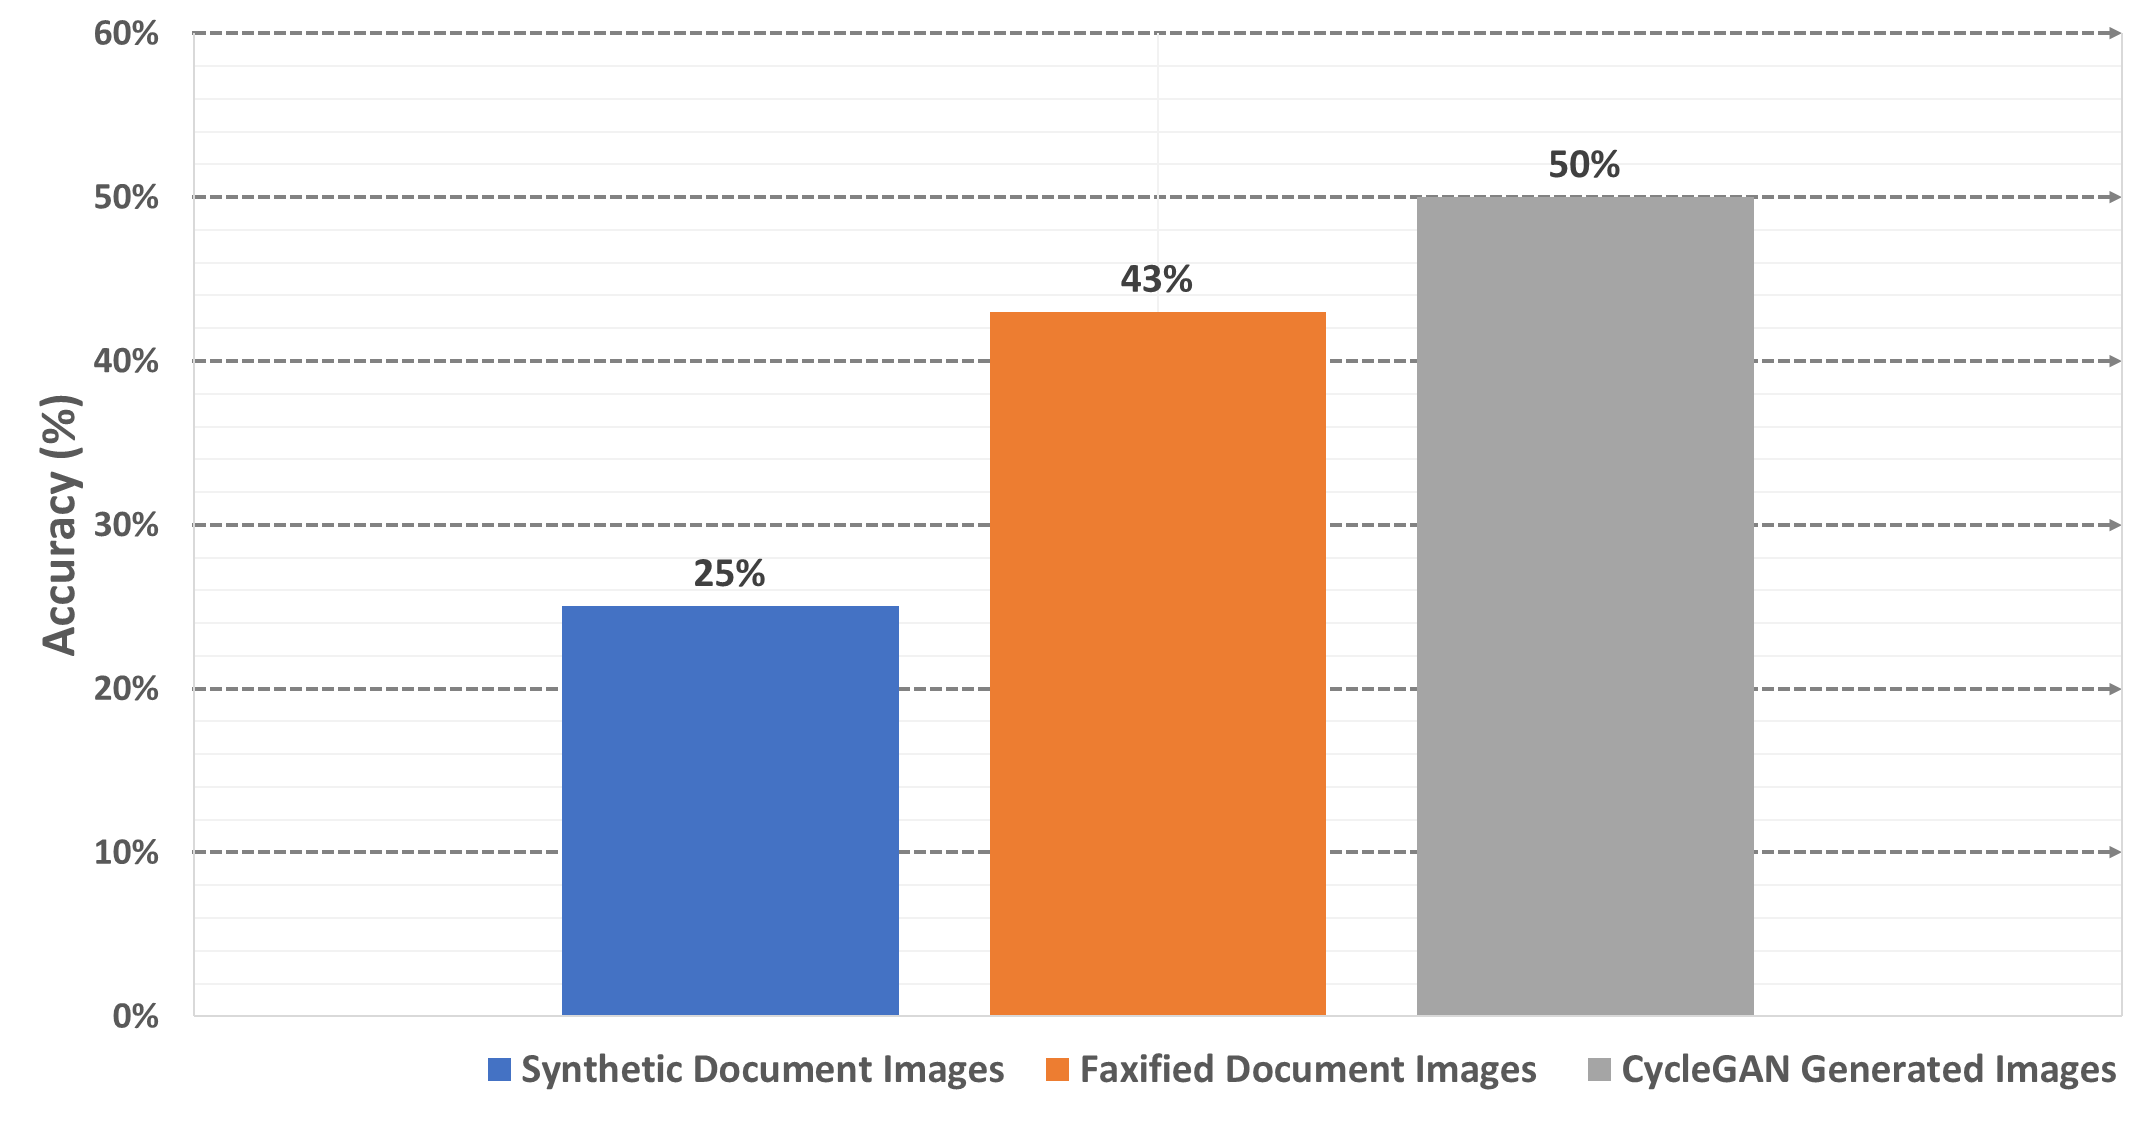
\includegraphics[scale=0.20]{images/DomainGap.png}
	    \caption[Illustration of Domain Gap Between Real Data Distribution and Synthetic Data Distribution, Faxified Data Distribution, and \ac{CycleGAN} Generated Data Distribution.]{Illustration of Domain Gap Between Real Data Distribution and Synthetic Data Distribution, Faxified Data Distribution, and \ac{CycleGAN} Generated Data Distribution. Initially, the classifiers are trained on Synthetic Document Images, Faxified Document Images, and \ac{CycleGAN} Generated Document Images. Later their Classification Performance Evaluated on the Annotated Real Document Images to understand the Domain Gap between distributions using Accuracy as an Evaluation Metric.}
	    \label{fig:DomainGap}
	    \end{center}
\end{figure}
\end{comment}








